\documentclass[11pt]{article}
\usepackage[latin1]{inputenc}
\usepackage{a4wide}
\usepackage{amsmath}
\usepackage{amsfonts}
\usepackage{amssymb}
\usepackage{graphicx}
\usepackage{enumerate}
\usepackage{epstopdf}
\usepackage{float}
\usepackage{multicol}
\usepackage{hyperref}
\epstopdfsetup{outdir=./images/}
\usepackage{subcaption}
\usepackage[table,xcdraw]{xcolor}

\renewcommand{\thesubsection}{(\alph{subsection})}
\newcommand{\floor}[1]{\lfloor #1 \rfloor}

\title{Natural Computing, Assignment 4}
\author{Dennis Verheijden - s4455770 \and Pauline Lauron - s1016609 \and Joost Besseling - s4796799}
\begin{document}
\maketitle

\section*{Combining, Bagging \& Random Forests}
\section{}
\subsection{}
\begin{itemize}
	\item 
	The probability that all three doctors give the correct answer is $ 0.8^3 = 0.512$. 
	\item 
	The probability that exactly 2 doctors make the right call is $0.8*0.8*0.2 + 0.8*0.2*0.8 + 0.2*0.8*0.8 = 0.384$. Therefore, the probability that \emph{at least} two doctors make the right call is $0.512 + 0.384 = 0.896$.
	\item  The probability that this group makes the right decision based on majority voting is $0.512 + 0.384 = 0.896$ since the majority is when there are at least two individuals. 
	%(Alternative approach, the probability that they all fail, and that exactly two doctors fail is ...)
\end{itemize}


\subsection{}
The general formula is 
\[
	P(\text{correct predictions with majority voting}) = \sum_{i = \floor{c/2}}^{c} p^{i} (1-p)^{c-i}  \binom{c}{i}.
\]

Using this formula, we find a probability of about $0.826$.

\subsection{}
If we use $10000$ runs of the simulations, we get an approximately equal result of $0.826$. Writing out more decimals gives us a difference of $0.0057$. So our approximation is pretty good.

\subsection{}
We decided to use a surfplot for the visualization. Here we can easily spot the differences when variables change relative to each other.

The surfplot can be found in figure \ref{fig:surf_probs}. What we can observe from this plot is that the jury size matters for a low number of people, but that this effect has exponentially diminishing returns. The competence, as expected, has the highest effect on the probability of correctly making the right decision.

\begin{figure}[H]
	\centering
	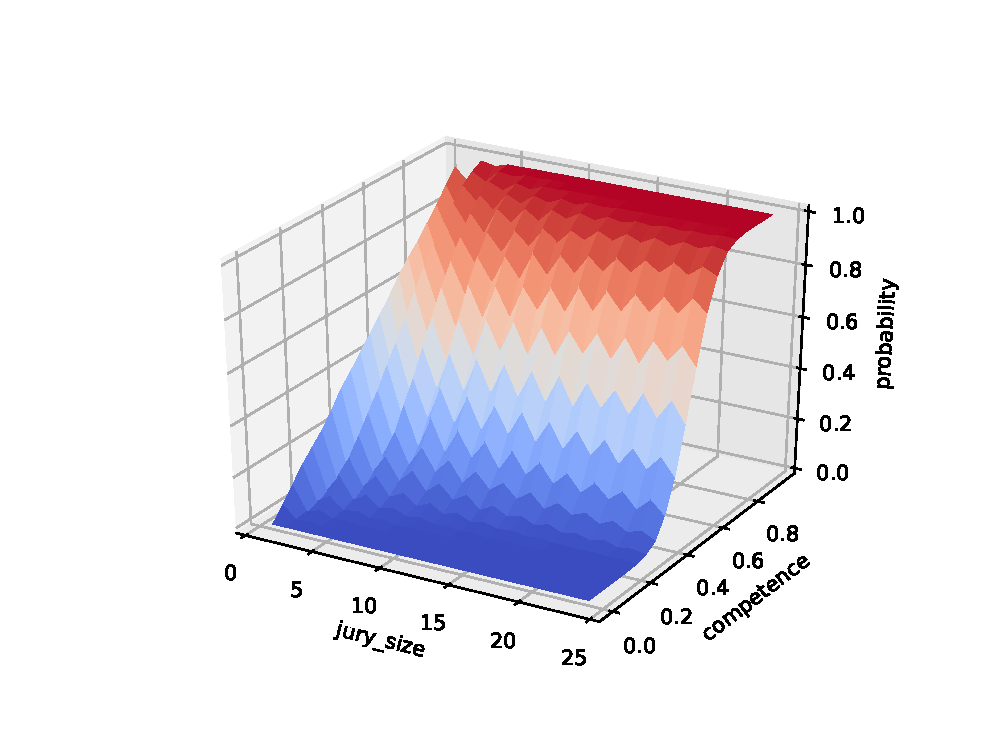
\includegraphics[width=0.75\textwidth]{images/surfplot_probs.eps}
	\caption{Surfplot of the probabilities as a function of the jury size $c$ and competence $p$.}
	\label{fig:surf_probs}
\end{figure}

\subsection{}
The probabilities for making the correct decision for the groups are:
\begin{itemize}
	\item \textbf{radiologists}: $0.850$
	\item \textbf{doctors}: $0.896$
	\item \textbf{students}: $0.826$
\end{itemize}
To reach the same probability for making the correct decision as the group of doctors, using only students. You would need 28 students. These would, collectively, have a probability of making the correct decision of $0.898$.

\section{}
The filled in table may be found below in table \ref{table:a}. Here we can see the values for different combinators.  Colors denote the choice that the classifier will make. What we can note from this table is that the choices of these classifiers are in most cases the same. 
\begin{table}[H]
	\centering
	\centering
	\begin{tabular}{ll|ll|ll|ll|ll|ll|ll}
		\multicolumn{2}{l}{$p_1(\omega|x)$} & \multicolumn{2}{l|}{$p_2(\omega|x)$} & \multicolumn{2}{l|}{$p_3(\omega|x)$} & \multicolumn{2}{l|}{Mean}                                 & \multicolumn{2}{l|}{Max}                                  & \multicolumn{2}{l|}{Min}                                  & \multicolumn{2}{l|}{Prod}                                     \\ \hline
		A                & B                & A                 & B                & A                 & B                & A                           & B                           & A                           & B                           & A                           & B                           & A                             & B                             \\ \hline
		0.9              & 0.1              & 0.9               & 0.1              & 0.0               & 1.0              & \cellcolor[HTML]{F8A102}0.6 & 0.4                         & 0.9                         & \cellcolor[HTML]{F8A102}1.0 & 0.0                         & \cellcolor[HTML]{F8A102}0.1 & 0.0                           & \cellcolor[HTML]{F8A102}0.01  \\
		0.9              & 0.1              & 0.9               & 0.1              & 0.3               & 0.7              & \cellcolor[HTML]{F8A102}0.7 & 0.3                         & \cellcolor[HTML]{F8A102}0.9 & 0.7                         & \cellcolor[HTML]{F8A102}0.3 & 0.1                         & \cellcolor[HTML]{F8A102}0.243 & 0.007                         \\
		0.9              & 0.1              & 0.2               & 0.8              & 0.1               & 0.9              & 0.4                         & \cellcolor[HTML]{F8A102}0.6 & \cellcolor[HTML]{FD6864}0.9 & \cellcolor[HTML]{FD6864}0.9 & \cellcolor[HTML]{FD6864}0.1 & \cellcolor[HTML]{FD6864}0.1 & 0.018                         & \cellcolor[HTML]{F8A102}0.072 \\
		0.0              & 1.0              & 0.0               & 1.0              & 0.0               & 1.0              & 0.0                         & \cellcolor[HTML]{F8A102}1.0 & 0.0                         & \cellcolor[HTML]{F8A102}1.0 & 0.0                         & \cellcolor[HTML]{F8A102}1.0 & 0.0                           & \cellcolor[HTML]{F8A102}1.0  
	\end{tabular}
	\caption{Classifier Combination for different methods. Values indicated in orange denote the decision the combiner would make. Values indicated in red denote a tie, the choice here is based on the implementation.}
	\label{table:a}
\end{table}

\section{}
The formula for the percentage of items that are not in a sample using Bootstrapping is:
\[
	p_{notPresent} = (1 - \frac{1}{N})^N
\]
We also made simulations which approximate this function, as found in figure \ref{fig:approx_vs_real}. Here we see that our simulations approximate our formula. Which adds evidence to its correctness.

Now that we have this implementation, we can also make simulations for different $N$. The results for this are shown in figure \ref{fig:leftout}. Here we can see a comparisons for choosing different values for $N$. We see that the probability of items that do not occur converge to $0.37$ for larger $N$. The last thing we can note is that there appears to be an exponential relation to the probability and $N$ as the probability first rapidly increases to $0.25$ for $N = 2$ and at $N=5$ it is almost at convergence.

\begin{figure}[H]
	\centering
	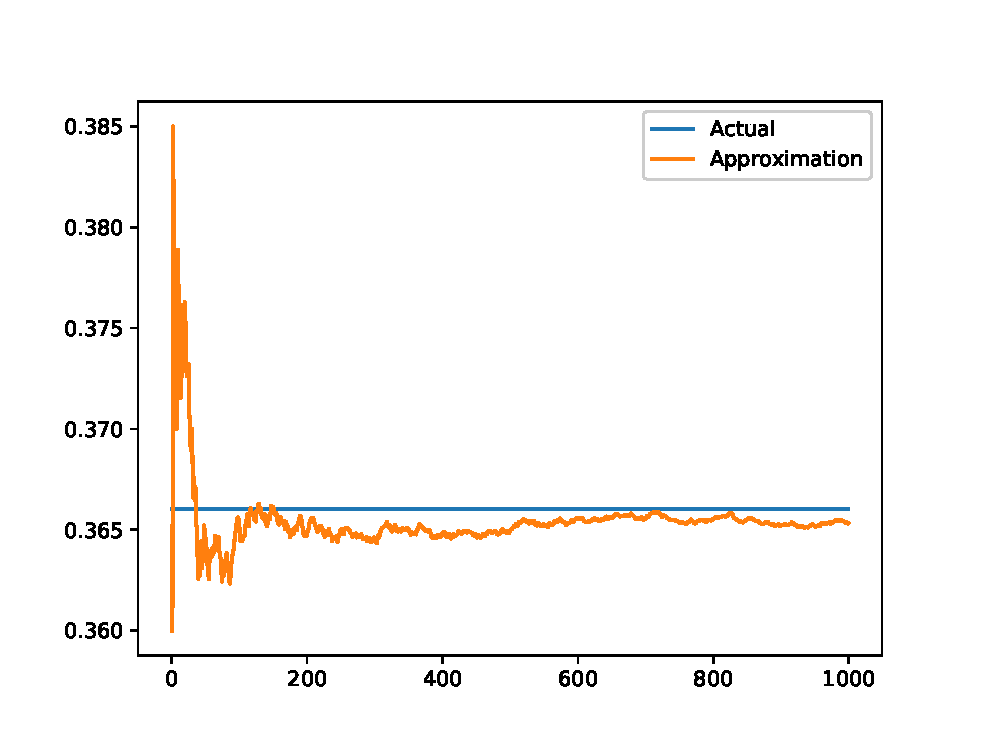
\includegraphics[width=0.7\textwidth]{images/approx_vs_real.eps}
	\caption{Comparison of our simulation and the exact value.}
	\label{fig:approx_vs_real}
\end{figure}

\begin{figure}[H]
	\centering
	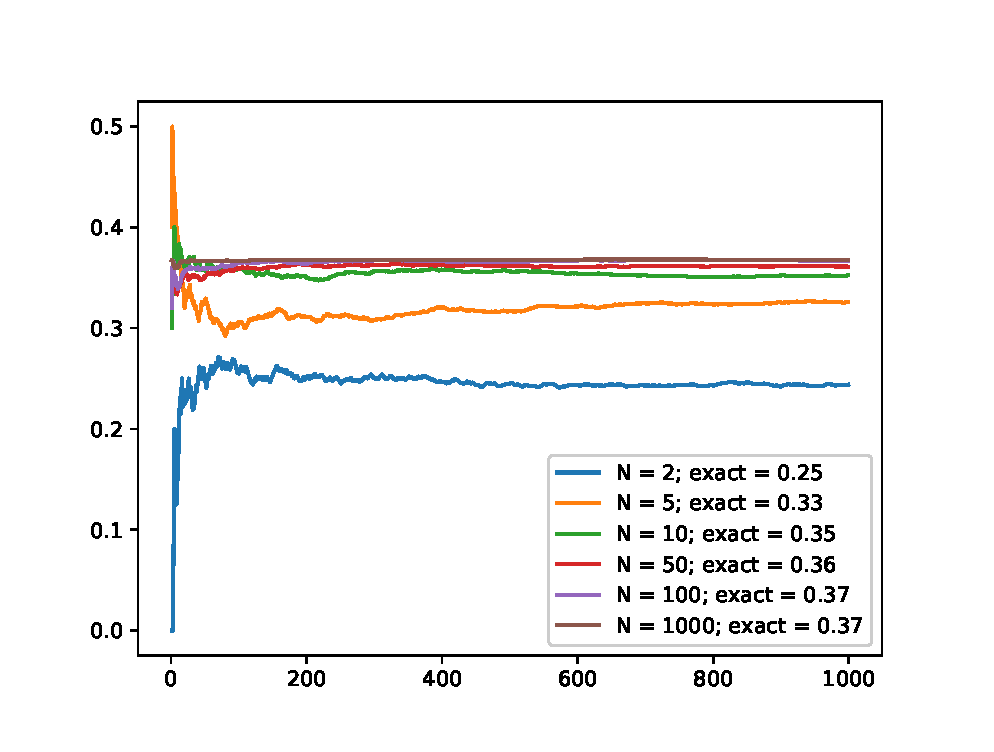
\includegraphics[width=0.7\textwidth]{images/different_sample_sizes.eps}
	\caption{Comparison of different sample sizes for the percentage of left-out items.}
	\label{fig:leftout}
\end{figure}

\section{}
The difference between bootstrapping and random subspaces is how the training data is constructed. 
\begin{itemize}
	\item In bootstrapping, you randomly select data from the whole dataset with replacement. Such that you can have samples that occur more than once.
	\item In random subspaces, you randomly select features from the whole dataset. So instead of randomly drawing samples, you draw features from these samples.
\end{itemize}


\section{}
We found multiple scores that are used to calculate variable importance. The first is the Mean Decrease Impurity, this basically calculates how well the set is divided based in each node, because each node only splits on one feature, we can use that to calculate a score.

The other measure is the Mean Decrease Accuracy (MDA). This is calculated by shuffling the contents of one feature in the dataset and keeping the other features the same. After that we calculate the decrease in accuracy. If the feature is not important, than shuffling it shouldn't change the accuracy much. If it is very important, the accuracy should get close to random chance. 

A disadvantage of the MDA is that it might not work correctly when the dataset is not balanced. If have 9 samples of class X, and 1 sample of class Y. And a feature that exactly determines whether a samply belongs to class Y. Shuffling on that feature will only decrease the accuracy by 0.1, but the feature is actually very important for class Y!
%critics : http://blog.datadive.net/selecting-good-features-part-iii-random-forests/

\section{}

~\\
For this experiment we used the handwritten digits, aka MNIST, dataset. As this dataset is easy to interpret and it has a decent difficulty to learn as the dataset contains 64 features and 10 classes.

We used the standard \texttt{RandomForestClassifier} from the python module \texttt{sklearn}. We found two variables that we thought to be important: \textit{max\_depth}, \textit{n\_estimators} and \textit{max\_features}. These respectively mean the maximum depth of a tree, the number of trees that are trained in the forest and the maximum number of features Random Forest is allowed to try in individual tree. The result of manipulating the first two parameters are found in figure \ref{fig:mnist_results}.

What we can note from this figure, is that both parameters converge. The default value for \textit{n\_estimators} is $10$. This value is roughly the value for which the algorithm converges. The default value for \textit{max\_depth} is not set, i.e. it expands until all leaves are pure or contain less than 2 samples. To better see whether setting this value is helpful, we can examine the results for certain values of the \textit{max\_depth} while leaving the parameter \textit{n\_estimators} to the default value. The results may be found in figure \ref{fig:mnist_lines}. What we can observe is that for a max tree depth of $1$ or $2$ the RandomForestClassifier is already way above chance, being $0.1$. The performance peaks at a max tree depth of 10. After this it starts to decline. This is because the tree is overfitting on the training set, which is an easy pitfall of this type of classifier. However, since it is an ensemble, the damage of overfitting is limited.
If we increase the max\_features, we supposed to have a better performance. However, if we used to much features, this will decrease the diversity of individual tree and we want don't want dependence between trees to have l tree in order to have better performance. 

To test different combination of parameters, we use the Grid Search. We obtain a score around 0.96. The best found parameters are while using logarithm function to calculate how many features should be covered, a max\_depth of 20 and 50 for the n\_estimators. These results can also be observed in figure \ref{fig:mnist_results} and \ref{fig:mnist_lines}, where more trees lead to a more stable accuracy and the max\_depth decreases for higher maximum depths.

Conclusion, setting the parameter \textit{n\_estimators} might not be necessary, depending on the domain. However, more estimators lead to more stable predictions. The parameter \textit{max\_depth} however, should be carefully set, as it has the most effect on the mean accuracy of the RandomForestClassifier.

\begin{figure}[H]
\centering
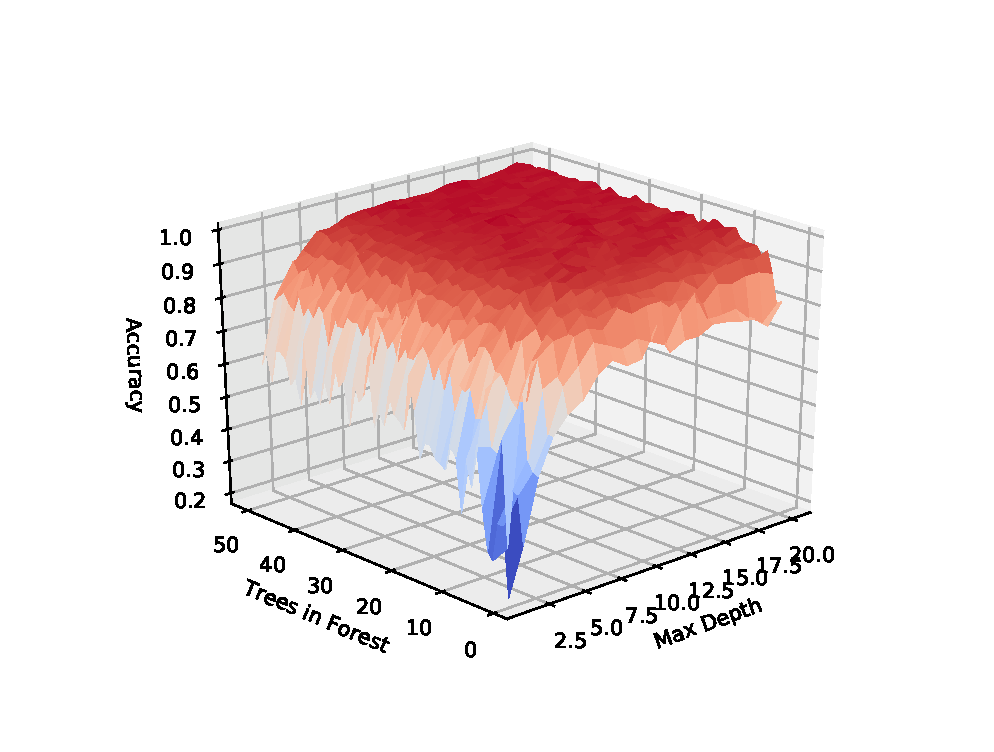
\includegraphics[width=0.7\textwidth]{images/mnist_results.eps}
\caption{The mean accuracy of RandomForstClassifiers for different parameter setups.}
\label{fig:mnist_results}
\end{figure}

\begin{figure}[H]
\centering
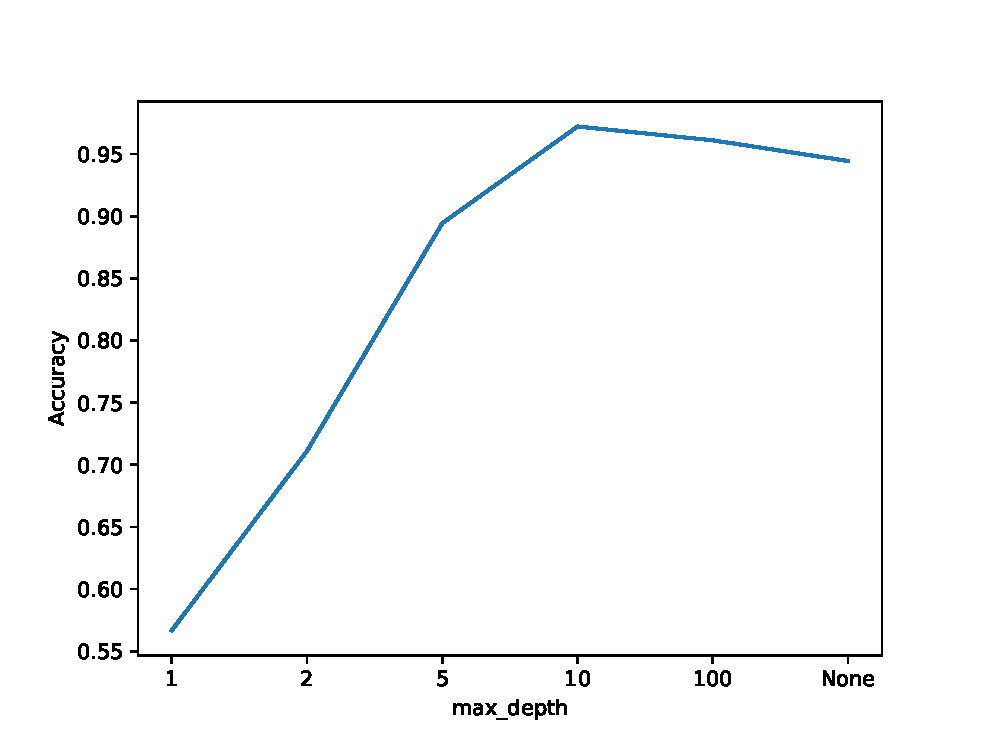
\includegraphics[width=0.7\textwidth]{images/mnist_lines.eps}
\caption{The mean accuracy of RandomForstClassifiers for choices for the max depth of the trees. The number of trees is set to the default value of $10$. A tree depth of \textit{None} means that the tree is allowed to split until the leaf nodes are either pure or have less than 2 samples.}
\label{fig:mnist_lines}
\end{figure}

\section*{Boosting}

\section*{1}

Derive the following weight:
\begin{align}
	\beta_m &= \frac{1}{2} \log \frac{1-\text{err}_m}{\text{err}_m} \\
	\intertext{where}
	\text{err}_m &= \frac{\sum_{i=1}^N w_i^{(m)} I(y_i \neq G_m(x_i))}{\sum_{i=1}^N w_i^{(m)}}
\end{align}

Plugging equation (10.11), which we will denote as $G$ into (10.9) gives:
\begin{align}
\beta_m &= \arg \min_\beta \sum_{y_i=G}^N w_i^{(m)} e^{\beta} + \sum_{y_i \neq G}^N w_i^{(m)} e^{-\beta}
\end{align}
To solve this we set the derivative to zero:
\begin{align}
\frac{d}{d\beta_m} \sum_{y_i=G}^N w_i^{(m)} e^{\beta_m} + \sum_{y_i \neq G}^N w_i^{(m)} e^{-\beta_m} &= 0\\
\sum_{y_i=G}^N w_i^{(m)} e^{\beta_m} - \sum_{y_i \neq G}^N w_i^{(m)} e^{-\beta_m} &= 0\\
e^{2\beta_m} &= \frac{\sum_{y_i \neq G}^N w_i^{(m)}}{\sum_{y_i=G}^N w_i^{(m)}}\\
2 \beta_m &= \log \frac{\sum_{y_i \neq G}^N w_i^{(m)}}{\sum_{y_i=G}^N w_i^{(m)}}\\
\beta_m &= \frac{1}{2} \log \frac{\sum_{y_i \neq G}^N w_i^{(m)}}{\sum_{y_i=G}^N w_i^{(m)}}\\
\beta_m &= \frac{1}{2} \log \frac{\sum_{i=1}^N w_i^{(m)} - \sum_{y_i \neq G}^N w_i^{(m)}}{\sum_{y_i=G}^N w_i^{(m)}}\\
\beta_m &= \frac{1}{2} \log \frac{\frac{1}{\sum_{i=1}^N w_i^{(m)}} \sum_{i=1}^N w_i^{(m)} - \sum_{y_i \neq G}^N w_i^{(m)}}{\frac{1}{\sum_{i=1}^N w_i^{(m)}} \sum_{y_i=G}^N w_i^{(m)}}\\
\beta_m &= \frac{1}{2} \log \frac{1 - \frac{\sum_{y_i \neq G}^N w_i^{(m)}}{\sum_{i=1}^N w_i^{(m)}}}{\frac{\sum_{y_i=G}^N w_i^{(m)}}{\sum_{i=1}^N w_i^{(m)}}}\\
\intertext{Now we can expand the summation $\sum_{y_i=G}$ in the fraction:}
\beta_m &= \frac{1}{2} \log \frac{1 - \frac{\sum_{i=1}^N w_i^{(m)} I(y_i \neq G_m(x_i))}{\sum_{i=1}^N w_i^{(m)}}}{\frac{\sum_{i=1}^N w_i^{(m)} I(y_i \neq G_m(x_i))}{\sum_{i=1}^N w_i^{(m)}}}\\
\intertext{Finally, we substitute $\frac{\sum_{i=1}^N w_i^{(m)} I(y_i \neq G_m(x_i))}{\sum_{i=1}^N w_i^{(m)}}$ back for the definition in (2):}
\beta_m &= \frac{1}{2} \log \frac{1-\text{err}_m}{\text{err}_m}
\end{align}

\section*{2}

\begin{figure}[h]
	\centering
	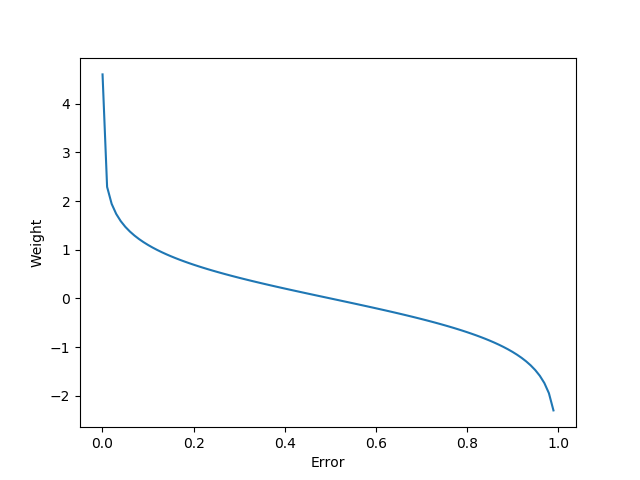
\includegraphics[width=0.6\textwidth]{images/ex2_2}
	\caption{A plot of the weight against the error}
\end{figure}
As the error goes to 0, the weight goes to infinity. When the error increases to 0.5, the weight of the learner slowly goes to 0, since a learner with a 0.5 error rate doesn't tell us anything about the data. 

If the error increases even further, $err>0.5$, the weight goes negative. This makes sense, because the truth is the opposite of the prediction of the classifier. We can use these results to improve our ensemble method.

If the learners are weak learners, the weight will be between 0 and 1.

\section*{3}

In bagging we train multiple learners by sampling from the dataset with replacement. We combine them by, for example, taking the average decision, or using a majority vote.

In boosting, we also train multiple learners, but use the learners to weight the samples from the dataset, such that samples that we predict wrong early on, get a higher weight. We combine the learners similarly to the boosting case, but we weight them according to their results on the training set.

\section*{4}
Both methods train multiple classifiers, using the results of the intermediate classifiers to measure the importance of each sample. They then both give importance to the difficult instances. How this is done, sets Adaboost and Gradient Boosting apart.

\section*{5}

\begin{figure}[h]
	\centering
	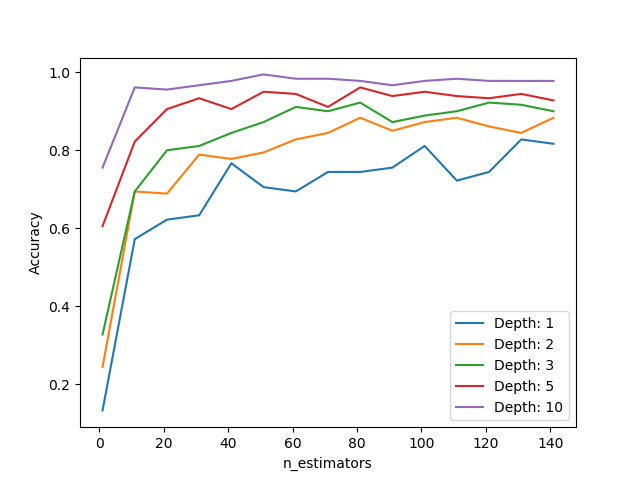
\includegraphics[width=0.6\textwidth]{images/ex2_5_depth_estimators}
	\caption{Adaboost using DecisionTreeClassifiers of varying depths. The accuracy is plotted as a function of the number of estimators (Trees) in the classifier.}
	\label{fig:acc_vs_ests}
\end{figure}
We used the same dataset as in the last exercise, because we want to compare the results. We used the sklearn implementation of the AdaBoostClassifier, combined with a DecisionTreeClassifier.  We used  $\texttt{max\_features}=\log_2$ for the decision tree.

Since AdaBoost is designed to use weak learners and combine them into a strong learner, we wanted to see how the strength of the individual learner influenced the strength of the combined learner. So we plotted the accuracy against the number of estimators \ref{fig:acc_vs_ests}, for 5 different decision trees, each with a higher allowed depth (increasing the strength of the learner). 

We can see that even the weakest possible learner manages to get an accuracy of around 0.8, although it needs many more estimators than the other learners to achieve this result. This shows us that the AdaBoost algorithm really manages to \emph{boost} the learners! Further we can see that having a stronger learner does improve the results.

If we look at the number of estimators, we can see that generally the improvement in accuracy is really high for the first 10 to 20, but after that they tend to plateau.

If we look at the learning rate in figure \ref{fig:lr}, we can see that the accuracy decreases really fast as it becomes larger. There is a big difference between the classifiers with a different number of estimators. The accuracy of the smallest classifier, with 10 estimators, goes down really fast. This is because the first estimator gives weights to `important' samples, but it might give high weights to samples that are not that important. Deteriorating the accuracy of the meta-classifier.
This effect is less strong when we have more estimators, because the later estimators can correct this result.


\begin{figure}[h]
	\centering
	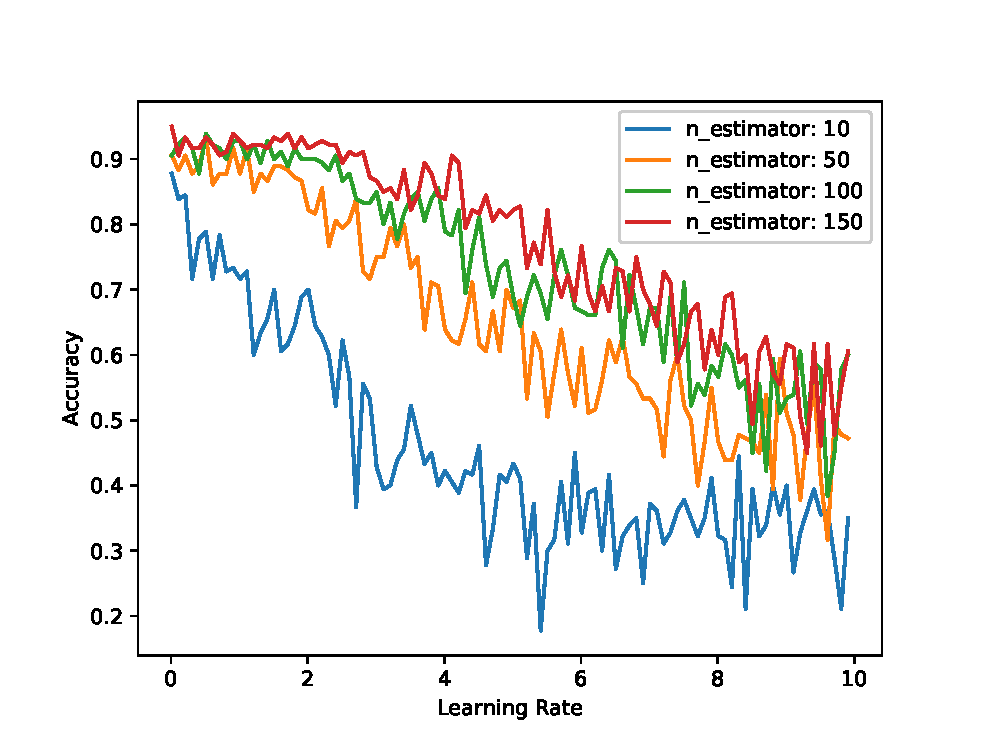
\includegraphics[width=0.6\textwidth]{images/ex2_5_lr_estimators.eps}
	\caption{Adaboost with Decision Tree Classifiers with a varying number of estimators. The accuracy is plotted as a function of the learning rate.}
	\label{fig:lr}
\end{figure}



\end{document}